\documentclass[../main]{subfiles}
 
\begin{document}

\chapter{Historical behavior}\label{cha:historical-behavior}

Ergodic theory tries to find order in chaos by showing that even if a dynamical system looks complicated, the statistical properties of its orbits are often well behaved. But what if the statistics don't even exist for most orbits? When this happens for all orbits starting in a set of positive reference measure, the phenomenon is known as \emph{non-statistical}, or \emph{historical} behavior.

More precisely, by existence of statistics, we mean the weak convergence of the empirical measures \(\Emp[n]{x} \weakto \mu\) to an asymptotic measure \(\mu\). To say that \((\Emp[n]{x})_n\) does not converge, therefore, is equivalent (in the compact setting) to the existence of a continuous observable \(\varphi \colon X \to \RR\) such that
\begin{equation}\label{eq:3}
  \lim_{n \to \infty} \frac{1}{n}\sum_{i = 0}^{n - 1} \varphi(f^i(x))
\end{equation}
does not exist.\footnote{The fact we don't need to quantify over measures that could be limits here is a consequence of \cref{cor:conv_of_exists}.} We then say that a diffeomorphism \(f\) of a compact manifold presents historical behavior if \(\Emp[n]{x}[spar, n]\) does not converge for \(x\) in a set of positive Lebesgue measure.

\section{History}
The ``historical'' terminology was introduced by Ruelle in~\cite{ruelleHistoricalBehaviourSmooth2001}, suggesting that for \cref{eq:3} not to converge, the sequence must keep ``changing its mind'' as \(n\) goes to infinity, and therefore has some sort of history. For instance, in the absence of external forces like human activity, we could expect that general patterns in climate would follow some predictable statistics, while with climate change we see that such statistics are not consistent along history. In the article, Ruelle recognized the problem of \textit{nonrecurrent} behavior of orbits as going against the expectation that recurrent behavior is generic in the space of diffeomorphisms, and presented the open problem of finding whether historical behavior can exist in a persistent manner, making some physical justifications for this possibility. He cites the theory of spin glasses, where the time evolution of the system is akin to a random walk in a random potential: a particle stays arbitrarily large amounts of time exploring some valley in the potential before eventually crossing the barrier to another valley, in such a way that time averages like \cref{eq:3} do not exist. As we shall see in this chapter, we can indeed produce historical behavior by constructing a diffeomorphism whose orbits behave like random walks, albeit not necessarily persistently.

Later, Floris Takens exposed the problem again in~\cite{takensOrbitsHistoricBehaviour2008}, giving some promising examples that were known at the time and also making some remarks about generiticity of points without asymptotic measures. For this reason and his work in related matters, the open question also became known as \textit{Taken's Last Problem}.

\begin{example}[Logistic family]
   The family of interval maps \(f_a(x) = ax(1 - x)\), for \(0 < a \le 4\), is known as the logistic family, and is one of the earliest examples where historical behavior is present abundantly: in~\cite{hofbauerQuadraticMapsAsymptotic1990}, the authors showed that for an uncountable number of parameters \(a\), Lebesgue almost every orbit in \([0,1]\) has no asymptotic measure.
\end{example}

\todo{figure}

\begin{example}[Bowen's eye]
  Another example was given by Bowen, although it's also not persistent. 
\end{example}

\todo{figure}


\subsection{Genericity of historical orbits}
\todo{Under relatively few hypothesis, historical orbits form a residual subset of the manifold}.

\label{sec:genericity}

\todo{\cite{carvalhoGenericityHistoricBehavior2021}}



\section{Martingale-coboundary decomposition}

% Even though \cref{thm:donsker} requires the random variables to be independent, we can still reach similar conclusions by requiring them to be co-homologous

The key idea for applying \cref{thm:donsker-martingale} in a dynamical system \((X,\mathcal{F},\mu,f)\), where \(\mu\) is a \(f\)-invariant probability, is finding a sub-\(\sigma\)-algebra \(\mathcal{G} \subseteq \mathcal{F}\) for which \(\varphi \in L^2(\mu)\) can be decomposed as a sum
\begin{equation}\label{eq:coboundary}
  \varphi = \varphi_0 + \phi \circ f - \phi
\end{equation}
such that \(\phi \in L^2(\mu)\), \(\varphi_0\) is \(\mathcal{G}\)-measurable and \(\eta = (\varphi_0 \circ f^{i - 1})_{i \geq 1}\) is a reversed martingale difference sequence. Indeed, this allows the transference of the weak invariant principle for the original \(\varphi\): let \(\xi = \rpar{\varphi \circ f^{i - 1}}_{i \geq 1}\), and notice that
\begin{equation*}
  \PSum[n,rv = \xi] = \PSum[n,rv = \eta] + \phi \circ f^n - \phi,
\end{equation*}
so
\begin{equation*}
  \DProc[n,rv=\xi]{x}{t}
  = \frac{\PSum[\floor{nt},rv=\xi]{x}}{\sqrt{n}} = \DProc[n,rv=\eta]{x}{t} + \frac{1}{\sqrt{n}} \big(\phi \circ f^{\floor{nt}} - \phi\big)(x).
\end{equation*}
It suffices to show that for \(\mu\)-almost every \(x\), the second term in the sum converges uniformly to zero (as a function of \(t\)). Given \(\varepsilon > 0\), we look at the sets \(B_n = \{ x :(\phi ^2 \circ f^n)(x) \geq n \varepsilon \}\). Since
\begin{equation*}
  \sum_{n = 1}^{\infty}\mu(B_n) = \sum_{n = 1}^{\infty}\mu(\set{\phi^2 \geq n \varepsilon}) = \int \floor{\phi^2/ \varepsilon} \;d\mu \leq \frac{1}{\varepsilon} \lVert \phi \rVert_2^2,
\end{equation*}
by Borel-Cantelli, \(\mu(\limsup_{n \to \infty}B_n) = 0\). If we take the intersection over \(k\) of the sets \(\liminf_{n \to \infty}B_n^{\complement}\) for \(\varepsilon = 1/k\), we get a full-measure set \(G\) with the property that for every \(x \in G\) and \(\varepsilon > 0\), there exists \(N\) such that \(n \geq N\) implies \(\frac{1}{\sqrt{n}}|\phi(f^n(x))| \leq \varepsilon\). Now, let \(M \geq N\) be big enough so that \(n \geq M\) implies \(\frac{1}{\sqrt{n}}|\phi(f^i(x))| \leq \varepsilon\) for all \(0 \leq i \leq N\). So for \(n \geq M\),
\begin{equation*}
  \sup_{t \in [0,1]}\frac{1}{\sqrt{n}} \big\lvert\phi \circ f^{\floor{nt}} - \phi\big\rvert(x) \leq 
  \max_{0 \leq i \leq N}\frac{|\phi \circ f^{i}(x)|}{\sqrt{n}} + 
  \max_{N \leq i \le n}\frac{|\phi \circ f^{i}(x)|}{\sqrt{i}} 
  \leq 2\varepsilon
\end{equation*}
as desired.

\subsubsection{Existence of martingale-coboundary decomposition}
From now on, we assume that \(\mu\) is an ergodic measure for \(f\).

\begin{theorem}\label{thm:decomposition-existence}
  Suppose \(\varphi \in L^2(\mu)\) and \(\mathcal{F}_j = f ^{-j}(\mathcal{F})\) are such that
  \begin{equation*}
    \sum_{n = 0}^{\infty} \lVert \CE[\mu]{\varphi, \mathcal{F}_j} \rVert_2 < \infty.
  \end{equation*}
  Then a decomposition as in \cref{eq:coboundary} exists. Moreover, this implies that
  \begin{equation*}
    \int \varphi \;d\mu = \int \varphi_0 \;d\mu = 0
  \end{equation*}
  and that the series in
  \begin{equation*}
    \sigma ^2 = \lVert \varphi_0 \rVert^2_2 = \lVert \varphi \rVert_2^2 + 2\sum_{n = 1}^{\infty} \int \varphi \cdot \varphi \circ f^n \;d\mu
  \end{equation*}
  converges absolutely. By the preceding arguments, if \(\varphi_0 \neq 0\) then \(\DProc[n,rv = \xi,spar,pf]\mu \weakto \sigma W\).
\end{theorem}

\begin{proof}
  \newcommand{\pp}{\phi^+}
  \newcommand{\pn}{\phi^-}
  We begin by writing \(\phi= \pn + \pp\), where \(\pp = \CE[\mu]{\phi, \mathcal{G}_0}\).
  
  \todo{write}
\end{proof}

\begin{remark}
  If \(\varphi\) was a coboundary \(\varphi = \phi \circ f - \phi\) to begin with, then it is clear that \(\PSum[n,rv = \xi] = \phi \circ f^n - \phi\), so the iterates of the skew product \(F(x,y) = (f(x), y + \varphi(x))\) satisfy
  \begin{equation*}
    F^n(x_0,y_0) = (f^n(x_0), \phi(f^n(x_0)) - \phi(x_0) + y_0) \subseteq \graph(\psi)
  \end{equation*}
  and are thus contained in the graph of \(\psi\), where \(\psi(x) = \phi(x) - \phi(x_0) + y_0\). In particular, \(F\) is not ergodic for \(\mu \otimes \Leb\).
\end{remark}

\begin{corollary}\label{cor:decay-implies-summable}
  Suppose \(\varphi\) is such that there exists a summable sequence \(c_n > 0\) satisfying
  \begin{equation*}
    \int (\psi \circ f^n) \varphi \;d\mu \leq \lVert \psi \rVert_2c_n
  \end{equation*}
  for all \(\psi \in L^2(\mathcal{G})\), where \(\mathcal{G}\) is as in \cref{thm:decomposition-existence}. Then
  \begin{equation*}
    \sum_{n = 0}^{\infty} \lVert \CE{\varphi, f^{-n}(\mathcal{G})} \rVert_2 < \infty.
  \end{equation*}
\end{corollary}

\begin{remark}
  The book~\cite{vianaStochasticDynamicsDeterministic2021} proves this condition is satisfied for smooth expanding maps, Hölder-continuous \(\varphi\) and \(\mathcal{G} = \mathcal{F}\), so this includes the \(f(x) = kx\) maps. The second condition is trivial when \(\mathcal{G} = \mathcal{F}\).
\end{remark}

\section{Historical behavior for skew products}

\NewObject\Fun\Mu{\mu}

Let \((X,\mu)\) be a Borel probability space, where \(X\) is compact and metrizable, and \(F \colon X \times I \to X \times I\) a skew product of the form
\begin{equation*}
  F(x,y) = (g(x),f_x(y))
\end{equation*}
where \(g \colon X \to X\) is ergodic and measure-preserving. Suppose there is a homeomorphism \(\gamma \colon I \to \RR[closure]\) and a measurable function \(p \colon X \to \RR\) such that, if we set \(t_x(y) = y + p(x)\), we have \[t_{x} \circ \gamma = \gamma \circ f_x\] for all \(x \in X\), where \(t_x\) is to be interpreted as the translation by \(p(x)\). 
\[
  \begin{tikzcd}
    I \arrow[d, "\gamma"]\arrow[r, "f_{x}"] & I \arrow[d, "\gamma"]\\
    \RR[closure] \arrow[r,"t_{x}"] & \RR[closure]
  \end{tikzcd}
\]
Since the \(t_x\) are translations, there is no loss of generality in assuming \(\gamma(0) = -\infty\), \(\gamma(1) = +\infty\) and \(\gamma\left(\frac{1}{2}\right) = 0\), so we shall adopt this convention for simplicity.

\begin{theorem}\label{thm:wip-historical}
  If the weak invariance principle is valid for the pair \((g, p)\), in the sense \(\DProc[n,rv = \xi,spar,pf]\mu \weakto \sigma W\) for \(\sigma > 0\) and \(\xi = (p \circ g^{i - 1})_{i \geq 1}\), then \(F\) has historical behavior. More specifically,
  \begin{equation}\label{eq:emp-closure}
    \set{\delta_-, \delta_+} \subseteq \set{e_n(x,y)}[n \in \NN, ']
  \end{equation}
  where \(\delta_- = \mu \otimes \delta_{0}\) and \(\delta_+ = \mu \otimes \delta_{1}\) and the limit points are taken in the weak* topology.
\end{theorem}

% \begin{figure}[h]
%   \centering
%   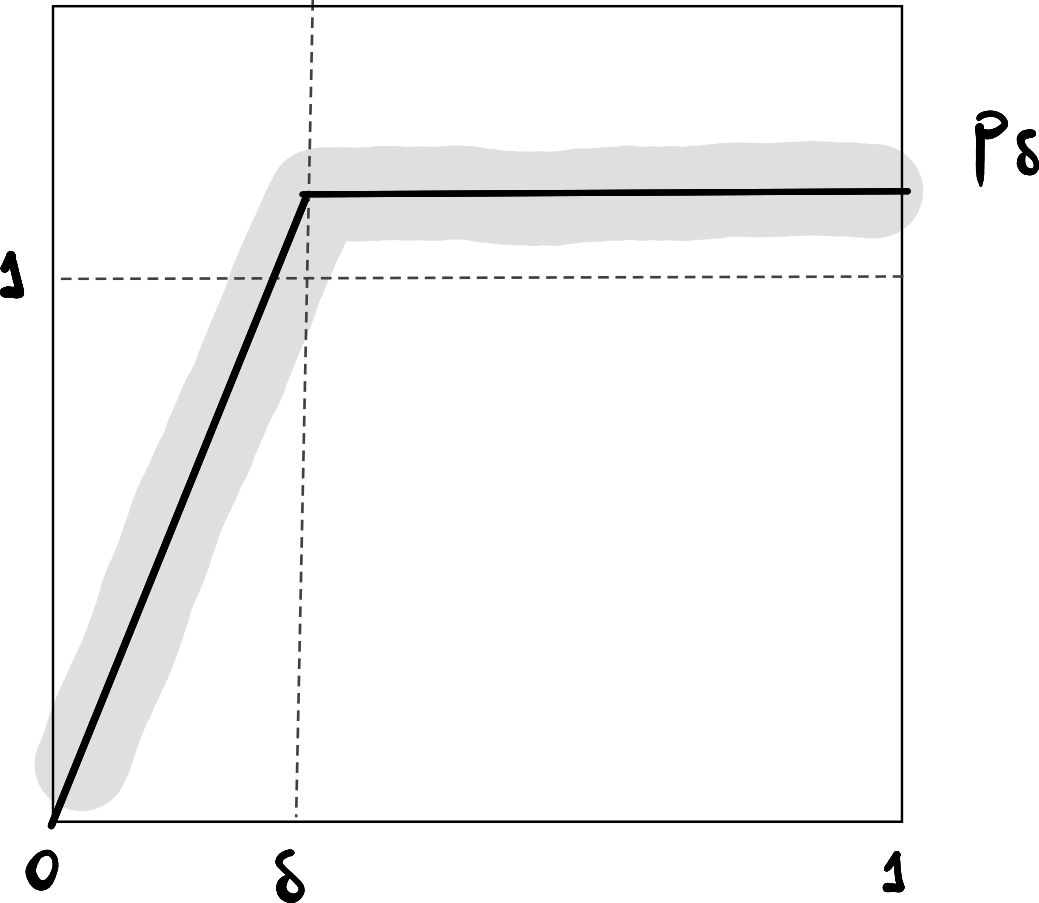
\includegraphics[width=5cm]{../figures/p-delta}
%   \caption{The function \(s_\delta\)}\label{fig:p-delta-plot}
% \end{figure}

\begin{proof}
  Let \(\delta > 0\) and \(s_{\delta} \colon [0,1] \to \RR\) be any continuous function such that \(s_{\delta}(0) = 0\) and \(s_{\delta}(t) > 1 + \delta\) for \(t > \delta\).
  Let \(U_{\delta} = B_{\delta}(s_{\delta})\) be an open ball of radius \(\delta\) around \(s_{\delta}\) in the uniform topology. By \cref{thm:forgery}, we know \(W(U_{\delta}) > 0\), so by \cref{thm:portmanteau}
  \begin{equation*}
    \liminf_{n \to \infty}(\DProc[n,spar,pf]\mu)(U_{\delta}) \geq \sigma W(U_{\delta}) > 0.
  \end{equation*}
  Therefore,
  \begin{equation*}
    S_{\delta} = \limsup_{n \to \infty}\, \DProc[n,spar,inv]{U_{\delta}} \subseteq X
  \end{equation*}
  has positive measure. This set is also invariant for \(g\) because
  \begin{align*}
    g^{-1}(S_{\delta})
    &= \limsup_{n \to \infty} \set{x \in X \where \DProc[n]{g(x)} \in U_{\delta}}\\
    &= \set[par = \Bigg]{x \in X : \liminf_{n \to \infty} \sup_t\abs*{\frac{\PSum[\floor{nt} + 1]{x} - p(x)}{\sqrt{n}} - s_{\delta}(t)} <\delta }\\
    &= \set[par = \Bigg]{x \in X : \liminf_{n \to \infty} \sup_t\abs*{\frac{\PSum[\floor{nt'}]{x}}{\sqrt{n}} - s_{\delta}(t)} <\delta }  \text{ where }t' = t + 1/n\\
    &= \set[par = \Bigg]{x \in X : \liminf_{n \to \infty} \sup_t\abs*{\frac{\PSum[\floor{nt}]{x}}{\sqrt{n}} - s_{\delta}(t)} <\delta } = S_{\delta}.
  \end{align*}
  Therefore \(\mu(S_{\delta}) = 1\). Now, notice that if \(x \in S_{\delta}\), then there is \(n_k^+ \to \infty\) for which for every \(k\), \(D_{n_k}^{\xi}(x) \in U_{\delta}\). This in turn implies that
  \begin{align*}
    \#\set[par = auto]{ 0 \leq i < n_k^+ \where S_{i}^{\xi}(x) > \sqrt{\textstyle n^+_k} } \geq (1 - \delta)n_k^{+}.
  \end{align*}
  Analogously, by repeating the argument with \(- s_{\delta}\), we find \(n_k^- \to \infty\) such that for every \(k\),
  \begin{align*}
    \#\set[par = auto]{ 0 \leq i < n_k^- \where S_{i}^{\xi}(x) < -\sqrt{\textstyle n^-_k} } \geq (1 - \delta)n_k^{-}.
  \end{align*}
  By considering \(E = \bigcap_{i = 1}^{\infty} U_{1/i} \subseteq X\), a set of full measure, and applying a diagonalization argument to the previous two observations, for each \(x \in E\) we find \(n_k^+, n_k^- \to \infty\) for which
  \begin{equation*}
    \frac{1}{n_k^+}\#\set[par = auto]{ 0 \leq i < n_k^+ \where S_{i}^{\xi}(x) > \sqrt{\textstyle n^+_k} } \to 1
  \end{equation*}
  and
  \begin{equation}\label{eq:6}
    \frac{1}{n_k^-}\#\set[par = auto]{ 0 \leq i < n_k^- \where S_{i}^{\xi}(x) < -\sqrt{\textstyle n^-_k} } \to 1.
  \end{equation}

  Now, by ergodicity of \(g\) and \cref{lem:erg-iff-basin-full-meas}, let \(S = E \cap \Basin{\mu}\) be a full measure set where
  \begin{equation*}
    \frac{1}{n} \sum_{i = 0}^{n - 1}\varphi(g^i(x)) \to \int_X \varphi(z) \;d\mu(z)
  \end{equation*}
  for all \(\varphi \in \Cs{X}\) and \(x \in S\).
  It suffices to show that for all \(x \in S\),
  \[e_{n^-_k}(x,y) \weakto \delta_- \quad\text{ and }\quad e_{n^+_k}(x,y) \weakto \delta_+.\]
  We only show the first convergence, since the second is analogous.

  Let \(\phi \in \Cs{X \times I}\) and \(\varepsilon > 0\). Since \(\phi\) is uniformly continuous, there is some \(k_1\) for which
  \begin{equation*}
    \sup\set[par = \big]{\abs{\phi(x,0) - \phi(x, s)} : x \in X, s \in [0,1/k_1]} < \varepsilon.
  \end{equation*}
  Let \(D = \set{i \where f^{(i)}_x(y) < 1/k_1}\), and let \(N\) be big enough so that for \(k \geq N\),
  \begin{equation*}
    \abs[\Bigg]{\frac{1}{n_k^-} \sum_{i = 0}^{n_k^- - 1}\phi(F^i(x,0)) - \int_X \phi(z,0) \;d\mu(z)} < \varepsilon,
  \end{equation*}
  which is possible since \(x \in \sS\) and \(\varphi(x) = \phi(x,0)\) is continuous, and also big enough so that
  \[\frac{1}{n_k^-}\# \set{ 0 \leq i < n_k^- \where i \notin D } < \varepsilon / \lVert \phi \rVert_{\infty},\]
  which is due to \cref{eq:6}. Therefore, we can estimate
  \begin{align*}
    \abs{e_{n_k^-}(x,y)(\phi) &- \delta_-(\phi)}\\
    &=
    \abs[\Bigg]{
    \frac{1}{n_k^-}\sum_{i = 0}^{n_k^- - 1} \phi(F^i(x,y))
      -
      \int_X \phi(z,0) \;d\mu(z)
      }\\
    &\leq
      \abs[\Bigg]{
      \frac{1}{n_k^-}\sum_{i = 0}^{n_k^- - 1} \phi(F^i(x,y))
      -
        \frac{1}{n_k^-}\sum_{i = 0}^{n_k^- - 1} \phi(F^i(x,0))
      } + \varepsilon
    \\
    &\le
      \frac{1}{n^-_k}
      \sum_{\substack{0 \leq i < n_k^- \\[1pt] i \in D}}
    \abs*{\phi(F^i(x,y)) - \phi(F^i(x,0))}
    +  \frac{2}{n^-_k}\sum_{\substack{0 \leq i < n^-_k \\[1pt] i \notin D}} \lVert \phi \rVert_{\infty} + \varepsilon\\
    &\le
      \frac{1}{n^-_k}
      \sum_{\substack{0 \leq i < n_k^- \\[1pt] i \in D}}
    \abs*{\phi(F^i(x,y)) - \phi(F^i(x,0))} + 3\varepsilon\\
    &\leq \varepsilon + 3\varepsilon = 4\varepsilon.
  \end{align*}
  This completes the proof.
\end{proof}


\begin{corollary}
  If for any compact \(K \subseteq \RR\), the vising time of the processes \(\PSum[n,rv = \xi]\) to \(K\) tends to zero almost surely as \(n \to \infty\), that is,
  \begin{equation*}
    \int 1_K \circ \PSum[n,rv = \xi](x)(t) \;d\Leb \to 0
  \end{equation*}
  then
  \begin{equation}\label{eq:4}
    \set{e_n(x,y)}[n \in \NN, '] = [\delta_-, \delta_+]
  \end{equation}
  for \(\mu\)-almost every \(x\) and all \(y \in (0,1)\).
\end{corollary}

\begin{proof}
  \begin{claim}
    If \(\eta \in \Meas{x,y}\), then \(\supp \eta \subseteq X \times \{ 0, 1 \}\) and \(\eta \in [\delta_-,\delta_+]\).
  \end{claim}

  
  We use \cref{lem:avoid-compacts} again for this. Let \(\Emp[n_k]{x,y} \weakto \eta\) be a limit point, \(x_0 \in X\) and \(y_0 \in (0,1)\), so there is a neighborhood \(\U\) of \((x_0,y_0)\) such that \(\U[closure] \subseteq X \times (0,1)\). By the lemma, \(\Emp[n_k]{x,y}(\U) \to 0\), so by \nameref{thm:portmanteau}
  \begin{equation*}
    \eta(\U) \leq \liminf_{k \to \infty} \Emp[n_k]{x,y}(\U) = 0.
  \end{equation*}
  This shows \((x_0,y_0) \notin \supp \eta\).

  We know \(\eta\) is a limiting measure for \(x\), so it is invariant by \(F\). The fact \(x \in S\) implies by the definition of \(S\) that \((\pi_1)_* \eta = \mu\). This means that \(\eta \ll \delta_- + \delta_+\), and since \(\delta_{ - }\) and \(\delta_+\) are ergodic measures, \(\eta\) must be a convex combination of the two.

  We have shown \(\Meas{x,y} \subseteq [\delta_-,\delta_+]\). To conclude \cref{eq:emp-closure}, it suffices to notice that by \cref{prop:limiting-measures}, \(\Meas{x,y}\) is connected, and therefore, since it contains both endpoints \(\delta_-\) and \(\delta_+\), it must be the whole segment.
\end{proof}


\section{Recent developments}

  \todo{Conclude with an overview of the recent work of Kiriri, Soma, Vargas et al.}

% \begin{theorem}
%   Under the same hypothesis as \cref{thm:wip-historical}, for every \(y \in (0,1)\),
%   \begin{equation}\label{eq:emp-convergence}
%     \Emp[n,spar,pf]{\mu\otimes \delta_y} \weakto \delta_*Z
%   \end{equation}
%   where \(Z\) is the arcsine measure on \([0,1]\) and \(\delta(\lambda) = \lambda\delta_- + (1 - \lambda)\delta_+\).
% \end{theorem}

% \begin{proof}
%   Let \(F \subseteq \Meas{X \times I}\) be a closed set, and let \(I = \delta([a,b]) = F \cap [\delta_-,\delta_+]\).

%   Idea: first, show that in \(I\) we get the desired statistics; then, show that in \(F \setminus I\) the times converge to zero.
% \end{proof}

% \subsection{Corollary: north-south maps}

% Consider some diffeomorphisms \(f_1, f_2, \dots, f_n \in \Diff[C^2]{I}\) preserving the orientation of the interval that commute with each other.

% such that \(f_+(y) > y\) and \(f_-(y) < y\) for all \(y \in (0,1)\).
% We first notice that we can always find 

% The covering map \(p\) is isomorphic to the usual covering map \(\pi \colon \RR \to \RR/\ZZ = \circl[upper = 1]\) via some homeomorphism \(h \colon \RR \to \I[int]\) such that \(\pi = p \circ h\)~\parencite[for instance,][Proposition 1.37]{hatcherAlgebraicTopology2002}.


% \begin{theorem}
%   Under the same hypothesis as \cref{thm:wip-historical}, for every \(y \in (0,1)\),
%   \begin{equation}
%     \F[upper = n, pf]{\Leb \otimes \delta_y} \weakto \frac{1}{2} (\delta_- + \delta_+).
%   \end{equation}
% \end{theorem}

% \begin{proof}
%   There is no loss of generality in assuming \(y = 0\).
%   Let \(\varphi \in \Cs{X \times I}\) and \(\varepsilon > 0\). From uniform continuity, there is \(M > 0\) for which \(\abs{\varphi(x, y) - \varphi(x,0)} < \varepsilon\) for all \(y < \gamma ^{-1}(-M)\) and \(\abs{\varphi(x, y) - \varphi(x,1)} < \varepsilon\) for all \(y > \gamma ^{-1}(M)\).

%   The evaluation functions \(\ev_t \colon \WPS \to \RR\) given by \(\ev_t(f) = f(t)\) are continuous \(W\)-almost everywhere, since \(W\) gives full measure to the set of continuous functions. By definition of the Wiener measure, \((\ev_t)_* W = \N[0][t]\), so the previous observation yields \((\ev_1 \circ \DProc[n])_* \mu \weakto \N[0][1]\). Let \(N\) for which \(n \geq N\) implies
%   \begin{equation*}
%     \N[0][1]\rpar*{\sqpar*{-\frac{M}{\sqrt{n}},\frac{M}{\sqrt{n}}}} \leq \varepsilon.
%   \end{equation*}
% \end{proof}


\ifSubfilesClassLoaded{
    \printbibliography
}{}

\end{document}
